\documentclass{llncs}
\usepackage[ruled,vlined]{algorithm2e}
\usepackage{color,graphicx,epstopdf,changepage,amsmath,multirow}

\SetAlgoCaptionSeparator{.\space}
\renewcommand\AlCapFnt{\normalfont\scshape}
\setlength{\algomargin}{0.7cm}

\title{A Particle Swarm Optimisation-Based Indirect Approach to Web Service Composition}

\author{Alexandre Sawczuk da Silva, Yi Mei, Hui Ma, Mengjie Zhang}
\institute{School of Engineering and Computer Science,
\\Victoria University of Wellington, New Zealand \\
\email{\{Alexandre.Sawczuk.Da.Silva, Yi.Mei, Hui.Ma, Mengjie.Zhang\}@ecs.vuw.ac.nz}}

\makeatletter
\usepackage[pdfauthor={\@author}, pdftitle={\@title}]{hyperref}
\makeatother

\providecommand{\e}[1]{\ensuremath{\times 10^{#1}}}

\begin{document}

\maketitle

\begin{abstract}
Web service composition has been an active research topic in the past years, as the prospect of having a system that automatically creates complex applications from building blocks (Web services) given some parameters is quite attractive to users. Existing approaches to automated composition rely on modifying and optimising solution structures directly, a complex process that requires several constraints to be considered before each alteration. In this work, a Particle Swarm Optimisation (PSO) with indirect composition representations is explored, using each particle to hold a service queue which is then decoded into a composition solution graph before fitness evaluation. This approach is compared to a previously proposed graph-based direct representation method, and experiment results show that the proposed approach produces solutions with greater or equivalent quality, even though its execution time is higher. Bar graphs showing the frequency with which each atomic service appears in a solution are also produced, indicating that the PSO-based approach explores a larger area of the search space.

\end{abstract}

\section{Introduction}

Software developers around the world are well acquainted with \textit{Web services}, which may be defined as applications that provide operations and/or data and are accessible via the network using communication protocols \cite{gottschalk2002introduction}. The advantage of these services lies in their modularity: they provide specific functionality that can be seamlessly integrated into larger applications, thus leading to code reuse and preventing time-consuming reimplementation \cite{dustdar2008services}. Indeed, the self-contained nature of Web services has led users to think of them as building blocks for more complex applications, selected and integrated as needed from a repository of available candidates in a process known as \textit{Web service composition} \cite{dustdar2008services}. As the number of candidates in the repository grows and as composition tasks become more complex, however, performing the selection and integration of services manually becomes increasingly difficult \cite{lecue2006formal}. Additionally, if the repository contains multiple candidates with equivalent functionality but different quality attributes, then manually choosing the ideal alternative to include in a composition may become infeasible \cite{gronmo2005model}. To overcome these challenges, researchers have been investigating the development of techniques to perform \textit{automated Web service composition} \cite{milanovic2004current}. By using these techniques, the \textit{composition requestor} would be able to simply specify the inputs and outputs of the desired application, and an \textit{automated composition system} would then correctly select and integrate services into a correct composition solution.

One important group of techniques to Web service composition focuses on creating a correct composition workflow, where atomic services are connected in a way that can be executed at runtime \cite{}. Another group focuses on optimising the quality of compositions, assuming that an abstract workflow is already known for the composition and then employing optimisation techniques to bind the best possible set of concrete services to this existing structure \cite{}. A third group of approaches attempts to address both of these concerns simultaneously, creating a correct workflow at the same time that it optimises the quality of the services included in the composition \cite{da2015graphevol}. However, simultaneously accomplishing these two tasks increases the complexity of these approaches, since the optimisation must also respect a number of interrelated constraints \cite{venkatraman2005generic}.

An alternative way to manage the complexity of addressing the simultaneous creation and optimisation of composition workflows is to optimise a set of heuristics that are then used for the construction of solutions, instead of directly optimising the actual compositions. This allows heuristics to be freely optimised, and constraints to be enforced once those heuristics are employed in the construction of a final solution. In this paper, a Particle Swarm Optimisation (PSO) \cite{eberhart2001particle} Web service composition approach that employs the strategy explained above is presented. More specifically, PSO is used to optimise the order of a queue of atomic services that is then provided to a graph-building algorithm. This algorithm uses the optimised queue to constructs composition solutions that abide by correctness constraints. The hypothesis is that this indirect optimisation approach will produce solutions that are equivalent to or better than direct optimisation approaches, while at the same time proposing a simpler composition approach.

The remainder of this paper is organised as follows: section \ref{background} provides the fundamental background on the Web service composition problem, including a literature review; section \ref{pso_approach} describes the PSO approach proposed in this paper; section \ref{experiment_design} describes the experiments conducted to test the performance of the novel PSO approach; section \ref{results} presents the results of these experiments; section \ref{conclusion} concludes the paper.

\section{Background}\label{background}

\subsection{Problem Description and Example}

The fundamental idea of Web service composition is to combine a set of modules, selected from a large pool of candidates, into a structure that accomplishes a more complex task. These modules are known as \textit{Web services}, and require a set of \textit{input} values in order to be executed, produce a set of \textit{output} values, and have an associated set of \textit{quality attributes} describing their non-functional aspects. The composition process must ensure that the Web services selected are compatible, and that the overall quality of the resulting solution is as high as possible. The fundamental elements in the composition problem are a \textit{service repository} containing the services, and a \textit{composition request} which specifies the overall inputs that should be made available when executing the composition as well as the overall outputs the composition should produce. The objective of this problem is to create a service composition with the best possible overall quality attributes, optimised according to a set of \textit{objective functions}, where each function is responsible for either maximising or minimising an aspect of the overall composition quality. There are three fundamental \textit{constraints} required in a composition solution: firstly, the inputs of each service in the composition must be a subset of the outputs provided by their predecessor services, meaning that the inputs of each service are fully satisfied; secondly, the outputs of the starting node of a composition must be the composition request’s overall inputs; thirdly, the inputs of the ending node of a composition must be the composition request’s overall outputs.

A classic Web service composition example the travel problem, which has been extensively described in the literature \cite{srivastava2003web,tang2010hybrid,sheng2014web}. In this scenario, the goal is to create a composite system that can book flights and accommodation at a given destination city according to the preferences specified by a user. More specifically, these overall composition inputs include the departure date and the destination city, and the overall composition outputs include reservation outcomes such as issued tickes and receipts. The services that make up the composition are selected from a pool of hotel and flight booking services that offer the desired elements of functionality with varying levels of quality, and structured into a workflow. Figure \ref{compositionExample} depicts an example of a composition solution for booking travel transport and accommodation. When using this system the customer provides the appropriate required input (i.e. their personal information, the origin and destination cities, the departure date, and the duration of the stay) and retrieves the desired output (i.e. issued tickets with a specific arrival date at the destination city).

\begin{figure}[h]
\centerline{
\fbox{
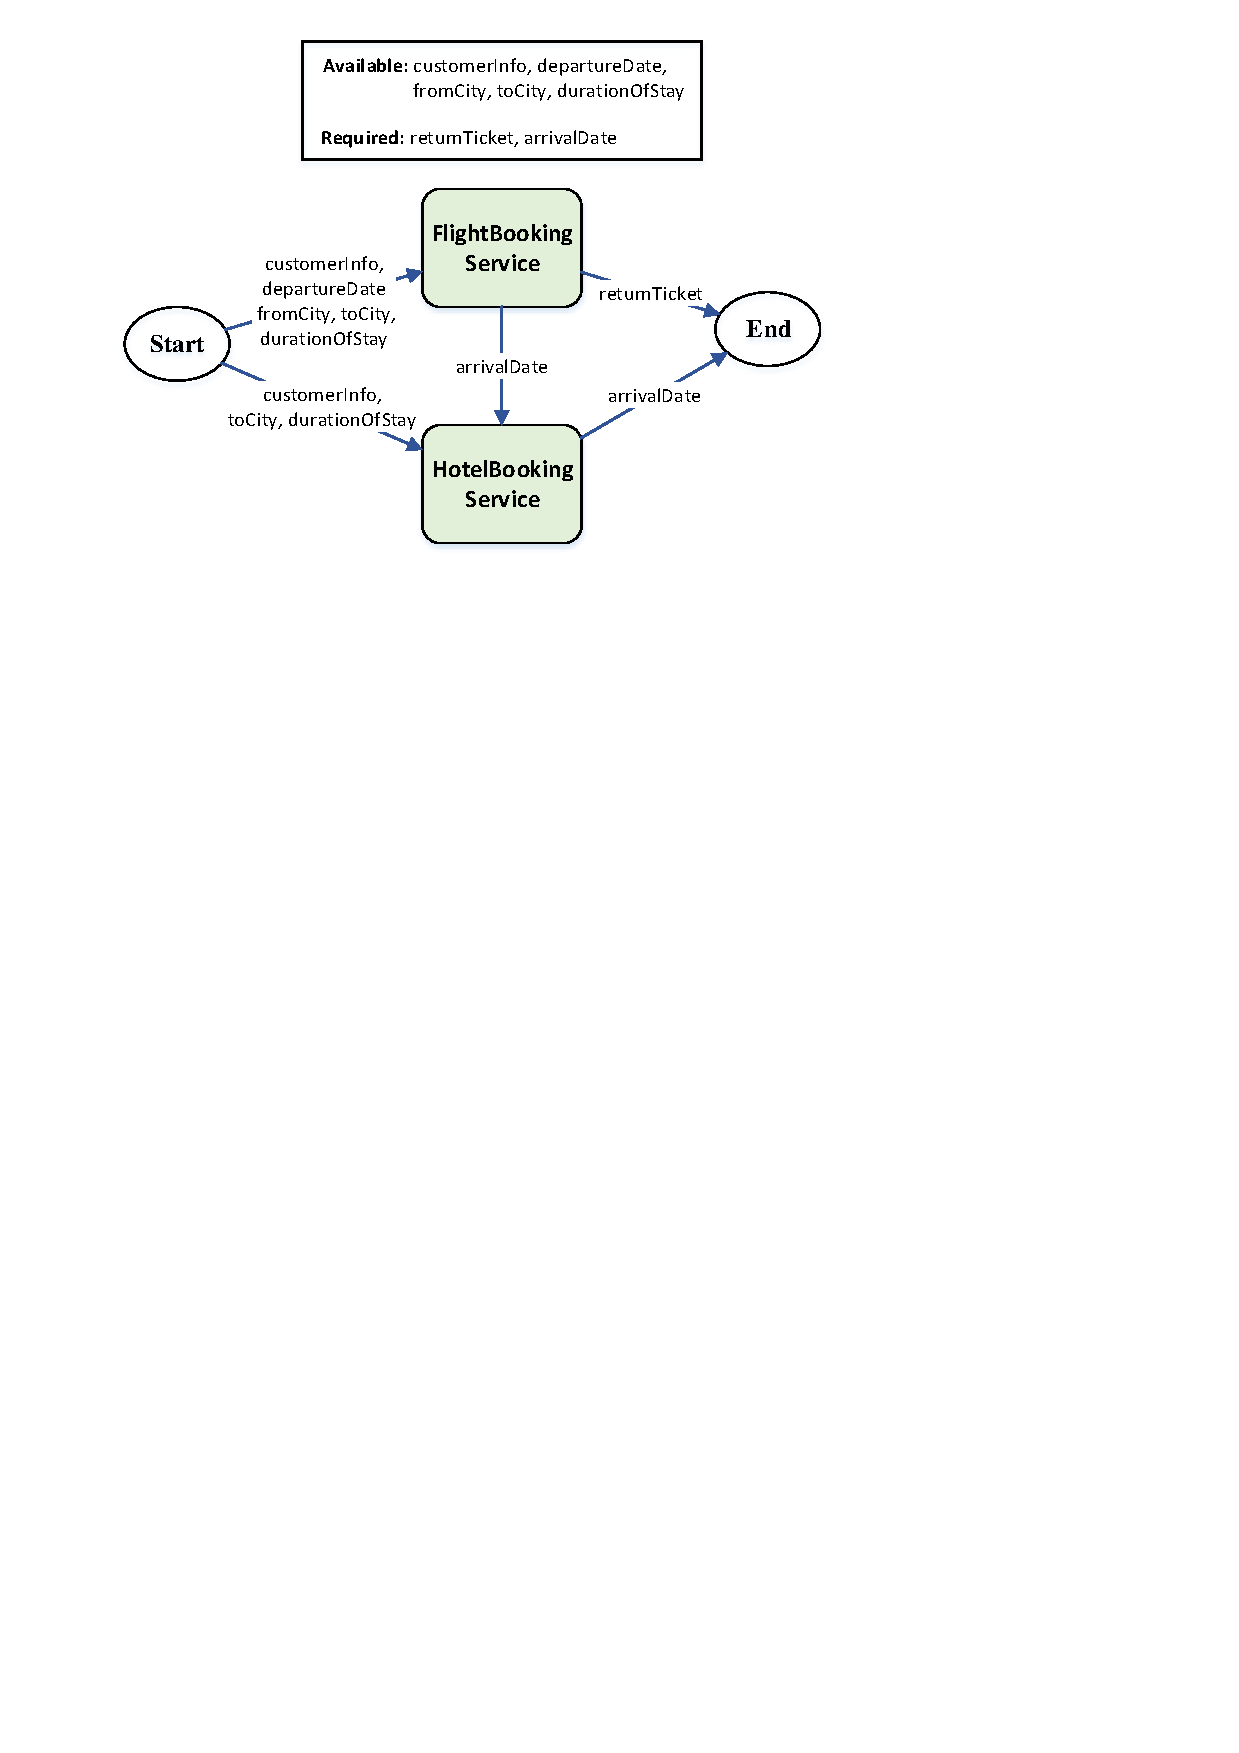
\includegraphics[width=8cm]{compositionExample.pdf}}}
\caption{Example of a solution to a Web service composition task \protect\cite{da2015graphevol}.}
\label{compositionExample}
\end{figure}

\subsection{Quality of Service and Composition Constructs}\label{qos_and_constructs}

When creating compositions, it is necessary to pay attention to the Quality of Service (QoS) properties of each selected service, i.e. a QoS-aware composition approach is needed. There exist many Web service quality properties, from security levels to service throughput \cite{menasce2002qos}. Based on the properties selected in previous works \cite{jaeger2007qos,yu2013adaptive}, in this paper we consider four of them: the probability of a service being available ($A$) upon request, the probability of a service providing a reliable response to a request ($R$), the expected service time limit between sending a request to the service and receiving a response ($T$), and the execution cost to be paid by the service requestor ($C$). The higher the probabilities of a service being available and of it producing a reliable response, the higher its quality with regard to $A$ and $R$; conversely, the services with the lowest response time and execution cost have the highest quality with regard to $T$ and $C$. The configuration of services in a composition is dictated by constructs used in building a workflow showing how services connect to each other \cite{zeng2003quality}. This work considers two composition constructs, sequence and parallel, that are recognised by Web service composition languages such as BPEL4WS\cite{yu2013adaptive,cardoso2004quality}. These two constructs are described as follows:

\begin{figure}[h]
\centerline{
\fbox{
\begin{tabular}{p{0.6\linewidth}}
\space\hfill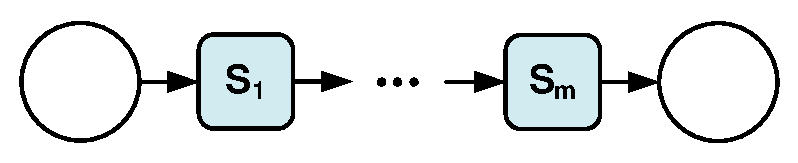
\includegraphics[width=2in]{sequence.eps}\hfill\space\\[0.2cm]
$T=\sum\limits^m_{n=1}t_n$ \hfill $C=\sum\limits^m_{n=1}c_n$ \hfill
$A=\prod\limits^m_{n=1}a_n$ \hfill $R=\prod\limits^m_{n=1}r_n$
\end{tabular}}}
\caption{Sequence construct and calculation of its QoS properties
\cite{yu2013adaptive}.}
\label{fig:sequence}
%\end{figure}
\vspace{0.3cm}
%\begin{figure}
\centerline{
\fbox{
\begin{tabular}{p{0.6\linewidth}}
\space\hfill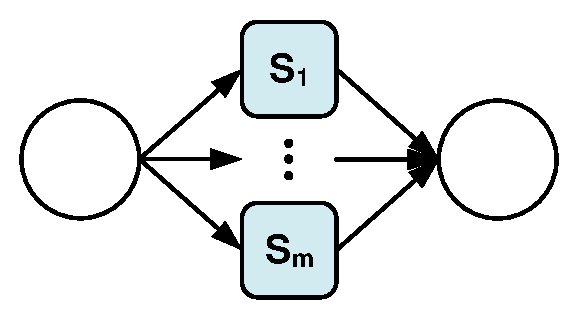
\includegraphics[width=1.4in]{parallel.eps}\hfill\space\\[0.2cm]
\space\hfill$T=MAX\{t_n|n\in\{1,\ldots,m\}\}$\hfill\space\\[0.2cm]
$C=\sum\limits^m_{n=1}c_n$ \hfill $A=\prod\limits^m_{n=1}a_n$ \hfill
$R=\prod\limits^m_{n=1}r_n$
\end{tabular}}}
\caption{Parallel construct and calculation of its QoS properties
\cite{yu2013adaptive}.}
\label{fig:parallel}
\end{figure}

\subsubsection{Sequence construct}
The component services of a sequence construct are executed in order, according to the edge flow. This makes the total time ($T$) and cost ($C$) of the sequence the sum of the value of those properties in each component service. As the availability ($A$) and reliability ($R$) of the sequence represent probabilities, they can be obtained by multiplying the value of those properties in each component service. This construct is shown in Figure \ref{fig:sequence}.
\subsubsection{Parallel construct} The components of a parallel construct are all executed simultaneously, since their incoming edges originate in a common node and their outgoing edges also converge to a common node. All QoS properties are calculated as for the sequence construct, except for the total time ($T$), which corresponds to that of the component service with the highest time. This construct is shown in Figure \ref{fig:parallel}.

\subsection{Particle Swarm Optimisation}

PSO is an optimisation algorithm based on the behaviour of social animals, such as a school of flying birds \cite{shi1998modified}. The core idea of PSO is to employ a swarm of particles that can communicate with each other to explore a search space and identify the best possible solution. Each particle holds a \textit{position} vector which specifies its current location in the solution space, and a \textit {velocity} vector that specifies the direction in which the particle is moving. Each particle also keeps track of the best solution location it has visited so far (i.e. its \textit{pBest}), and the whole swarm keeps track of the best overall location found so far (i.e. the \textit{gBest}). As explained in \cite{eberhart2001particle}, the original PSO process is divided into a number of steps, shown in Algorithm \ref{psoSteps}.

\begin{algorithm}[h]
 \setlength\hsize{0.9\linewidth}
 \SetKwInOut{Input}{Input}\SetKwInOut{Output}{Output}
 \let\oldnl\nl% Store \nl in \oldnl
\newcommand{\nonl}{\renewcommand{\nl}{\let\nl\oldnl}}
 \LinesNumbered
	\textbf{1.} Randomly initialise each particle in the swarm.\\
	\nonl \While {max. iterations not met}{
		\ForAll{particles in the swarm}{
			\textbf{2.} Calculate the particle's fitness.\\
			\eIf{fitness value better than pBest}{
				\textbf{3a.} Assign current fitness as new pBest.\\
			}{
				\textbf{3b.} Keep previous pBest.\\
			}		
		}
		\textbf{4.} Assign best particle's pBest value to gBest, if better than gBest.\\
		\textbf{5.} Calculate the velocity of each particle according to the equation:\\
		\Indp $v_{id} = v_{id} + c_1 * rand() * (p_{id} - x_{id}) + c_2 * rand() * (p_{gd} - x_{id})$\\
		\Indm \textbf{6.} Update the position of each particle according to the equation:\\
		\Indp $x_{id} = x_{id} + v_{id}$\\
	}
	
 \caption{Steps of the PSO optimisation technique.}
\label{psoSteps}
\end{algorithm}

The first step is to randomly initialise the position and velocity vectors of all particles in the swarm. Then, the following steps are repeated for the specified number of iterations: for each particle, the fitness value associated with its current location is calculated, and if it is better than the previous \textit{pBest}, then the \textit{pBest} is updated with it. Once the fitness has been calculated for all particles, we check whether the best particle's \textit{pBest} is better than the current \textit{gBest}, and we update \textit{gBest} if that is the case. We then update the velocity and position of each particle according to the equations listed in steps 5 and 6, respectively \cite{eberhart2001particle}. The equation for updating the velocity modifies each dimension in the velocity vector ($v_{id}$) by using the current local best ($p_{id}$), the current global best ($p_{gd}$), the current particle position ($x_{id}$), two user-defined coefficients ($c_1$ and $c_2$), and random variables ($rand()$); the equation for updating the positions uses the newly calculated velocity ($v_{id}$) to update each dimension of the position vector ($x_{id}$).

\subsection{Related Work}

A wide variety of Evolutionary Computing (EC) approaches has been applied to the problem of Web service composition, as evidenced by literature surveys of the field \cite{wang2012survey,pejman2012web}. One of the earliest works in this area \cite{canfora2005approach} applies genetic algorithms to optimise the overall Quality of Service (QoS) of a composition. The composition process in this work is \textit{semi-automated}, meaning that a workflow of abstract services has already been provided. In semi-automated compositions, the objective is to select a set of concrete services that fulfil the required functionality of their abstract counterparts, ensuring that the selected set results in a composition with the best possible quality. Even this approach takes QoS into account, it is not capable of performing \textit{fully automated} composition, which is when the composition workflow is automatically deduced at the same time that the services to include in the composition are identified.

* A semi-automated PSO approach to Web service composition (\cite{zhao2012improved})

Another approach \cite{rodriguez2010composition} employs Genetic Programming (GP) to perform fully automated Web service composition, representing solutions as a trees with candidate services as the leaf nodes and composition constructs as the inner nodes. A context-free grammar is used to generate new individuals at the beginning of the evolutionary process, as well as ensuring structural correctness during the crossover and mutation operations. Despite its favourable experimental results, this approach has the shortcoming of neglecting the Quality of Service of compositions, instead optimising candidates according to workflow topology measures such as the length of the longest path in the composition and the number of atomic services included.

* QoS-aware Web GP approach (use Yang's \cite{yu2013adaptive})

* GraphEvol approach \cite{da2015graphevol}


\section{PSO-Based Composition Approach}\label{pso_approach}
The aim of the PSO-based composition approach proposed in this paper is to optimise the queue of services used by a graph-building algorithm, which in turn determines the structure of the resulting composition. The rationale behind the creation of this method is that the indirect optimisation of the service queue allows for a simpler optimisation process than modifying composition solutions directly, while at the same time reducing the risk of creating an overly constrained search space. As Algorithm \ref{novelSteps} shows, this approach follows the usual PSO steps, though with some particularities. Firstly, the size of particles is determined based on the number of candidate services being considered for the composition, with each candidate service being mapped to an index of the particle's position vector (step 1). Secondly, solutions must be built using a graph-building algorithm before their fitness can be calculated; a queue of services is generated from the particle's position vector (step 3) and used as the input for the algorithm (step 4), which decodes a corresponding solution graph from it. Finally, the particle's fitness can be calculated from this corresponding solution graph (step 5). Further discussion on each of these highlighted steps is carried out in the subsections below.

\begin{algorithm}[h]
 \setlength\hsize{0.9\linewidth}
 \SetKwInOut{Input}{Input}\SetKwInOut{Output}{Output}
 \let\oldnl\nl% Store \nl in \oldnl
\newcommand{\nonl}{\renewcommand{\nl}{\let\nl\oldnl}}
 \LinesNumbered
 	\textcolor{blue}{\textbf{1.} Map each candidate service to an index in the particle's position vector.}\\
	\textbf{2.} Randomly initialise each particle in the swarm.\\
	\nonl \While {max. iterations not met}{
		\ForAll{particles in the swarm}{
		    \textcolor{blue}{\textbf{3.} Create queue of services using the particle's position vector.}\\
			\textcolor{blue}{\textbf{4.} Build the corresponding composition graph using the queue.}\\
			\textcolor{blue}{\textbf{5.} Calculate the fitness of the resulting graph.}\\
			\eIf{fitness value better than pBest}{
				\textbf{6a.} Assign current fitness as new pBest.\\
			}{
				\textbf{6b.} Keep previous pBest.\\
			}		
		}
		\textbf{7.} Assign best particle's pBest value to gBest, if better than gBest.\\
		\textbf{8.} Calculate the velocity of each particle according to the equation:\\
		\Indp $v_{id} = v_{id} + c_1 * rand() * (p_{id} - x_{id}) + c_2 * rand() * (p_{gd} - x_{id})$\\
		\Indm \textbf{9.} Update the position of each particle according to the equation:\\
		\Indp $x_{id} = x_{id} + v_{id}$\\
	}
	
 \caption{Steps of the PSO-based Web service composition technique.}
\label{novelSteps}
\end{algorithm}

\subsection{Particle Mapping (Step 1)}

As explained before, each particle in this approach represents a queue of candidate services, i.e. a queue of those services that can potentially be used to construct a solution that satisfies the composition request. However, before the optimisation process begins the service repository is run through a discovery process \cite{wang2013genetic} that identifies the subset of services that could possibly be used to create a composition. As shown in Algorithm \ref{discovery}, this filtering process requires the set of inputs ($I$) and the set of outputs ($O$) from the overall composition task, in addition to the service repository ($R$); given these inputs, it produces a list of candidate services that are relevant to the composition ($S_{list}$). The algorithm keeps track of all available inputs so far ($C_{search}$), and uses them to discover additional services: if a previously undiscovered service has all of its inputs satisfied by $C_{search}$, then it is added to $S_{list}$ and its outputs are added as available inputs in $C_{search}$. The discovery continues until no additional services are found, and the final step verifies whether the desired composite output $O$ can in fact be achieved using the services in the repository.

\begin{algorithm}
\setlength\hsize{0.9\linewidth}
 \SetKwInOut{Input}{Input}\SetKwInOut{Output}{Output}
 \LinesNumbered
 \SetNlSty{}{}{:}
 %\SetLine % For v3.9
 \Input{$I$, $O$, $R$}
 \Output{a list of services $S_{list}$}
 $C_{search} \leftarrow I$\;
 $S_{list} \leftarrow \{\}$\;
 $S_{found} \leftarrow DiscoverService()$\;
 \While{$|S_{found}| > 0$}{
  $S_{list} \leftarrow S_{list} \cup S_{found}$\;
  $C_{search} \leftarrow C_{search} \cup C_{output}$ of $S_{found}$\;
  $S_{found} \leftarrow DiscoverService()$\;
  }
  \eIf{$C_{search} \supseteq O$}{
   \Return $S_{list}$\;
   }{
   Report no solution\;
 }
\caption{Discovering relevant services for composition \cite{wang2013genetic}.}
\label{discovery}
\end{algorithm}

Once the relevant services within the repository have been identified, they are mapped to particles in the swarm following the principle depicted in Figure \ref{mapping}. Namely, each relevant service is mapped to a different index of the particle's position vector in a consistent manner, so that a given index value corresponds to the same service across the entire swarm. This means that the number of dimensions in a particle is determined dynamically, and it corresponds to the number of relevant services in the repository. Each cell in the the position vectors of all particles are randomly initialised with values between 0 and 1 (inclusive).

\begin{figure}[h]
\centerline{
\fbox{
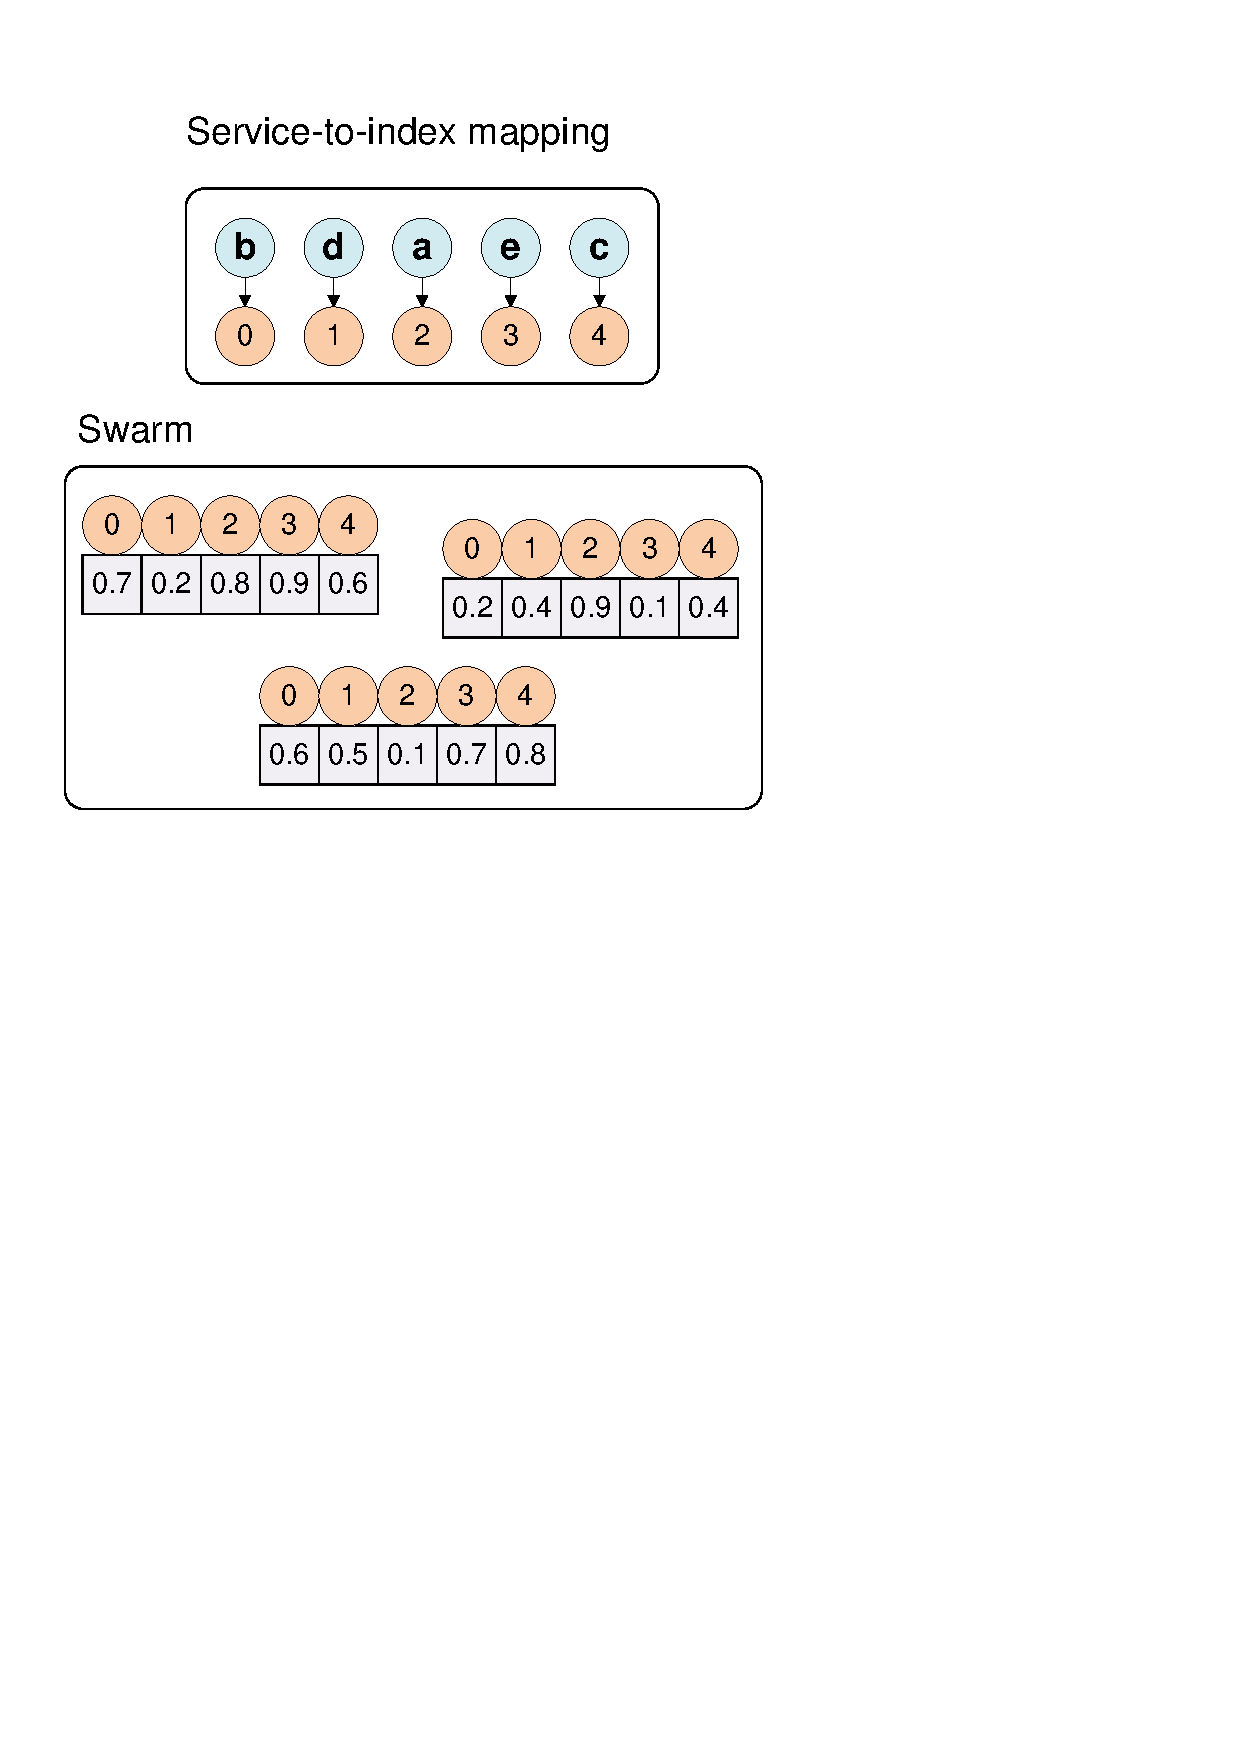
\includegraphics[width=6cm]{mapping.pdf}}}
 \caption{Mapping of relevant services to particles, and random initialisation.}
 \label{mapping}
\end{figure}

\subsection{Creation of Service Queue (Step 3)}

Before constructing a composition graph based on the information contained in a particle, it is necessary to construct a service queue using the particle's position vector. As shown in Figure \ref{queue}, this is done by checking the service-to-index mapping for the particles' position vector. Each relevant service is placed on the queue with an associated weight, which is retrieved by accessing the position vector with the index mapped to that service. This queue is then sorted according to these weights, placing the services with the highest weight at the head of the queue, and those with the lowest weight at the tail. Note that if two or more services have the same weight, then the ordering between them may vary.

\begin{figure}[h]
\centerline{
\fbox{
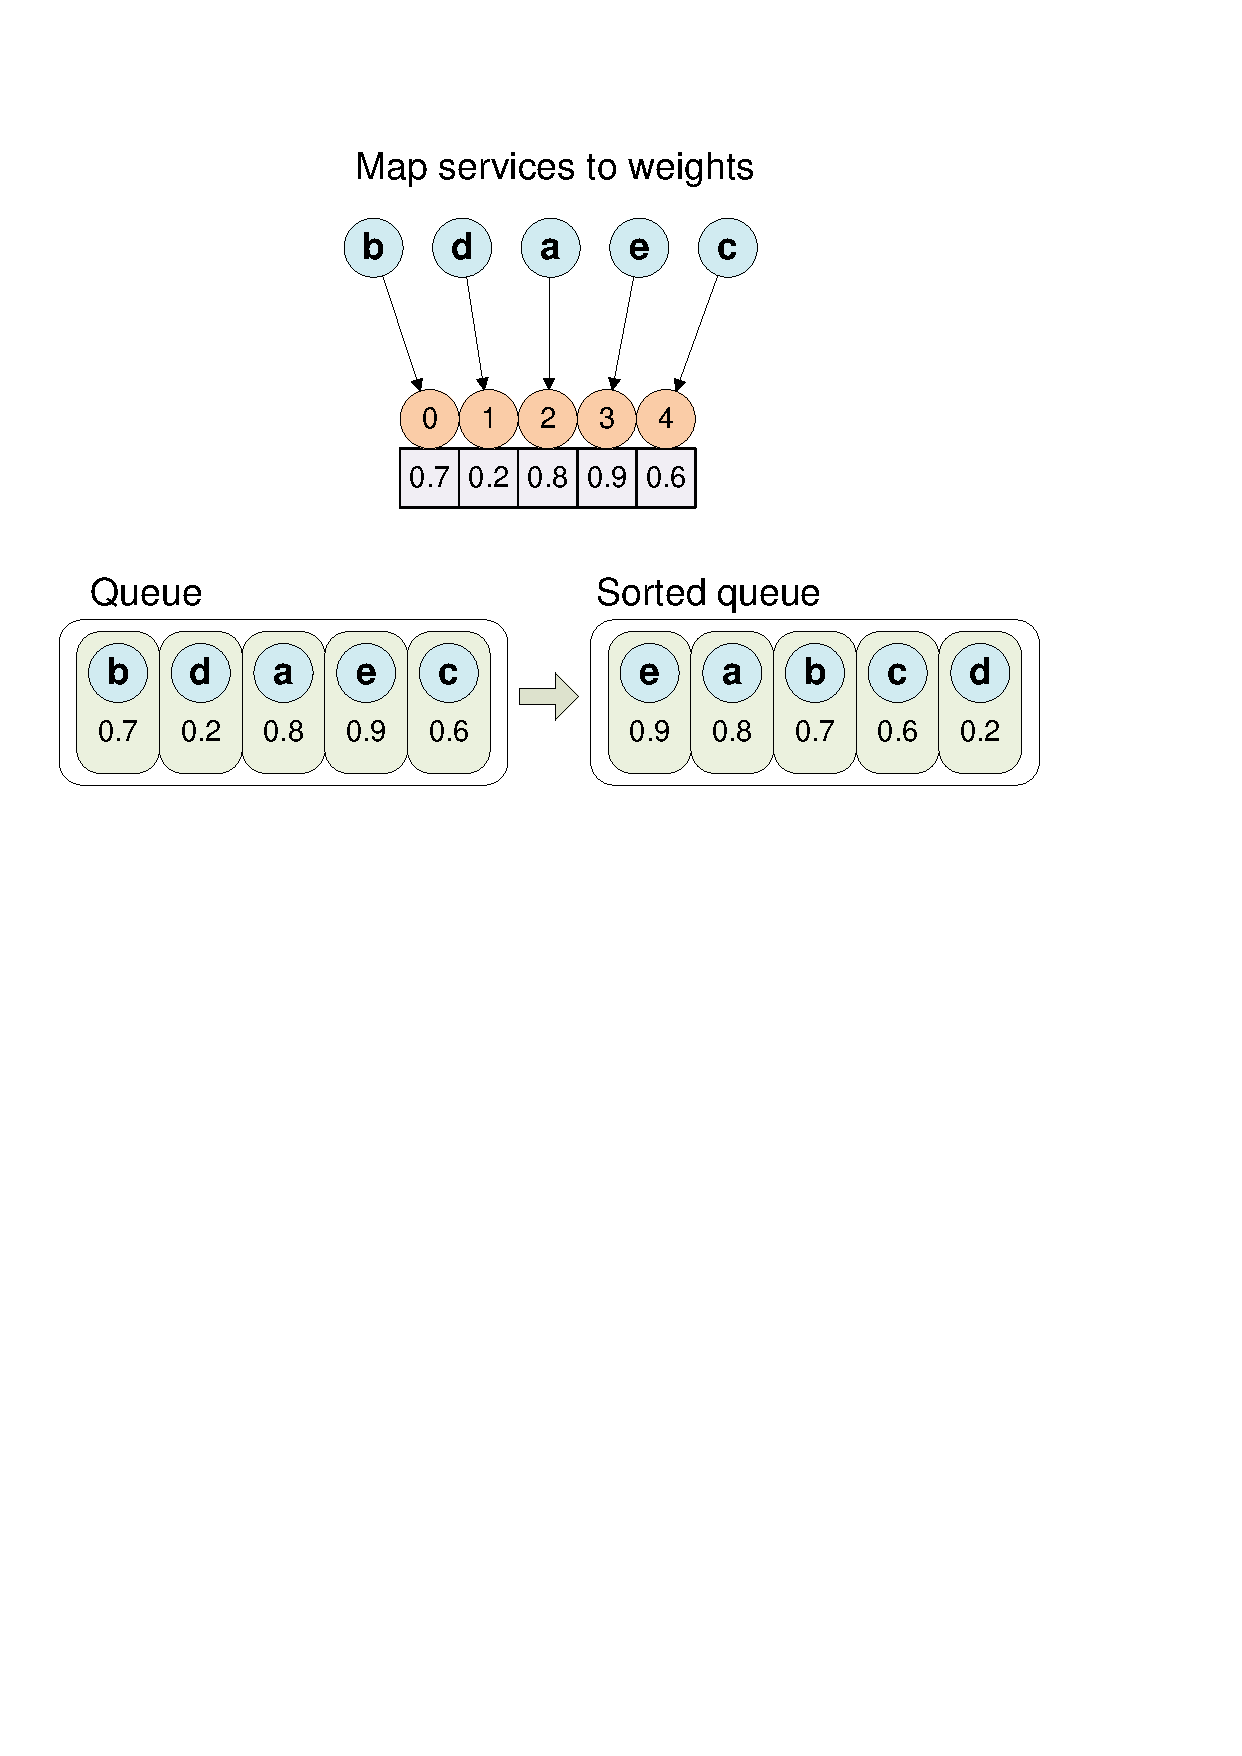
\includegraphics[width=8cm]{serviceQueue.pdf}}}
 \caption{Generating a service queue from a particle.}
 \label{queue}
\end{figure}

\subsection{Graph-Building Algorithm (Step 4)}

By determining the service queue represented in a particle, it is then possible to build a composition graph from that service ordering, based on the Graphplan technique discussed in \cite{blum1997fast}. The graph is built in a forward way -- from the $start$ node towards the $end$ node -- to prevent the formation of cycles, which may lead to the addition of nodes that do not contribute to reaching the $end$ (i.e. dangling nodes). To address this, after the graph has been constructed it is submitted to a function that removes these redundant nodes.

\begin{algorithm}[h]
 \setlength\hsize{0.9\linewidth}
 \SetKwInOut{Input}{Input}\SetKwInOut{Output}{Output}
 \SetKwFunction{connectNode}{connectNode}\SetKwFunction{findCands}{findCands}\SetKwFunction{removeDangling}{removeDangling}
 \LinesNumbered
 \SetNlSty{}{}{:}
 \Input{$I$, $O$, $queue$}
 \Output{composition graph $G$}
 $start.outputs \leftarrow \{I\}$\;
 $end.inputs \leftarrow \{O\}$\;
 $G.edges \leftarrow \{\}$\;
 $G.nodes \leftarrow \{start\}$\;
 $availOutputs \leftarrow \{start.outputs\}$\;
 $index \leftarrow 0$\;
 \While{$end.inputs \not\sqsubseteq availInputs$}{\label{buildingLine}
 $cand \leftarrow queue.get(index)$\;
 $index \leftarrow index + 1$\;
 \If{$cand.inputs \sqsubseteq availOutputs$}{
 \connectNode{$cand, G$}\;
 $currEndInputs \leftarrow availOutputs \cup \{cand.outputs\}$\;
 $queue \leftarrow queue.remove(index)$\;
 $index \leftarrow 0$\;
 }}
 \connectNode{$end, G$}\;
 \removeDangling{$G$}\;
 \KwRet $G$\;
 \vspace{2mm}
 \SetKwProg{myproc}{Procedure}{}{}
 \myproc{\connectNode{$n, G$}}{
   $inputsToFulfil \leftarrow \{cand.inputs\}$\;
 \While{$|inputsToFulfil| > 0$}{
	$graphN \leftarrow G.nodes.next()$\; 
	\If{$|n.inputs \sqcap graphN.outputs| > 0$}{
	  $inputsToFulfil \leftarrow inputsToFulfil - (n.inputs \sqcap graphN.outputs)$\;
	  $G.edges \leftarrow G.edges \cup \{graphN \rightarrow n\}$\;
    }
    $G.nodes \leftarrow G.nodes \cup \{n\}$\;
 }}
 \caption{Generating a composition graph from a queue.}
\label{graph_building}
\end{algorithm}

 As shown in Algorithm \ref{graph_building}, the values initially required are the composition task inputs ($I$), task outputs ($O$), and a $queue$ of services as its input; this leads to the creation of a composition graph $G$. We begin by assigning $I$ as the set of outputs produced by the graph's $start$ node, and $O$ as the set of input nodes required by the graph's $end$ node. Then, $start$ is added to the graph $G$, its outputs are added to a set ($availOutputs$) that records all available outputs from the nodes currently in the graph, and an $index$ variable is created to track positions in the $queue$ (holding 0, which indicates the queue head). After this setup stage, the following steps are repeated until $availOutputs$ can be used to fulfil all of the inputs of $end$: the node at the current $queue$ position ($index$) is retrieved as a candidate ($cand$); if all of its inputs can be fulfilled, $cand$ is connected to the graph using $connectNode$ -- which works by identifying existing nodes in the graph whose output fulfils the input of $cand$, and creating connecting edges from these existing nodes to $cand$ --, its outputs are added to $availOutputs$, it is removed from the queue, and $index$ is reset to 0; otherwise, the candidate in the next queue position is considered. Once all $end$ node inputs can be fulfilled, $end$ is connected to the graph, any dangling nodes are removed, and $G$ is returned. In summary, by using this algorithm the structure of the resulting graph changes depending on the service ordering within the queue provided as input.

\subsection{Fitness Calculation (Step 5)}

The fitness for a candidate graph is calculated using a function that evaluates its overall QoS values, considering the four attributes discussed in subsection \ref{qos_and_constructs}. The QoS attributes are combined using a weighted sum, according to the following function for a graph $i$:

\begin{equation}
fitness_i = w_1A_i + w_2R_i + w_3(1 - T_i) + w_4(1 - C_i)
\end{equation}

\noindent where $\sum_{i=1}^{4} w_i = 1$
\\\\
$A$, $C$, and $R$ are calculated using each atomic service in the graph according to the formulae shown in Figures \ref{fig:sequence} an \ref{fig:parallel}; $T$, on the other hand, is determined by adding the individual times of the services that form the longest path in the graph, from start to end. The time is calculated based on the longest graph path because this allows us to handle both parallel and sequence constructs at the same time. The output of the fitness function is within the range [0, 1], with 1 representing the best possible fitness and 0 representing the worst. To ensure that the final result of the sum is within this range, the values of $A$, $C$, $R$ and $T$ must all be normalised between 0 and 1. This is done by identifying the minimum and maximum values for each QoS attribute within the the dataset, then using the following formula (applied individually for each of the four quality attributes):

\begin{equation}
normalise(value) = 
\begin{cases}
	\frac{value - min}{max - min} & \text{ if }max - min \neq 0.\\
	1 & \mathrm{ otherwise}.
\end{cases}
\end{equation}

\section{Experiment Design}\label{experiment_design}

Experiments were conducted to evaluate the performance of the PSO-based indirect composition approach in comparison to a graph-based direct composition approach \cite{da2015graphevol}, according to three criteria. The first criterion is execution time, with the hypothesis that the graph-based approach will take less time to execute than the PSO-based approach; the second criterion is best solution fitness, with the hypothesis that the solutions provided by the PSO-based approach will match or surpass the quality of those produced by the graph-based approach; the third criterion is search space coverage, with the hypothesis that the PSO-based approach will consider a greater variety of solutions during the search process than the graph-based approach. If these hypotheses are shown to be true, the implication is that the PSO-based is a suitable Web service composition alternative when prioritising the exploration of the search space.

\subsection{Parameters}

All experiments were conducted on a personal computer with 8 GB RAM and and an Intel Core i7-4770 CPU (3.4GHz). The datasets and tasks from WSC-2008 \cite{bansal2008wsc} and WSC-2009 \cite{kona2009wsc} were used to compare the graph-based and PSO-based approaches, with 30 independent runs for each approach using each dataset. The choice of the parameters used for executing each approach, shown in Table \ref{tab:parameters}, was based on common settings from the literature \cite{koza1992genetic,eberhart2001particle}.

\begin{table}[h]
\centering
\caption{Parameters used for experiments.}
\label{tab:parameters}
\begin{tabular}{|c|c|c|c|}
\hline
\multicolumn{2}{|c|}{{\bf Graph-based}} & \multicolumn{2}{c|}{{\bf PSO-based}} \\ \hline
Population size        & 500            & Swarm size          & 30             \\ \hline
Generations            & 51             & Iterations          & 100            \\ \hline
Fitness weights        & 0.25 (all)     & Fitness weights     & 0.25 (all)     \\ \hline
Mutation prob.         & 0.8            & $c_1$               & 1.49618        \\ \hline
Crossover prob.        & 0.1            & $c_2$               & 1.49618        \\ \hline
Reproduction prob.     & 0.1            & $w$                 & 0.7298         \\ \hline
Tournament size        & 2              &                     &                \\ \hline
\end{tabular}
\end{table}

\section{Results}\label{results}

Results showing the execution time and solution fitness of the graph-based and the PSO-based approaches are displayed in Table \ref{tab:results}, where the first column indicates the dataset used, the second and third columns contain the mean execution time and mean fitness (respectively) of the PSO-based approach, and the fourth and fifth columns contain the time and fitness of the graph-based approach. All values are shown in 2dp, and means are accompanied by the standard deviation. A Wilcoxon signed-rank test at .95 confidence interval was conducted to ascertain whether the differences between the results for the two approaches are statistically significant, and the symbols $\uparrow$ and $\downarrow$ are used to indicate significantly larger and significantly smaller values, respectively. 

\begin{table}[h]
\centering
\caption{Execution time and fitness results for PSO and graph-based composition approaches.}
\label{tab:results}
\begin{tabular}{|c|c|c|c|c|}
\hline
\multirow{2}{*}{{\bf Dataset}} & \multicolumn{2}{c|}{{\bf PSO-based}}               & \multicolumn{2}{c|}{{\bf Graph-based}}                     \\ \cline{2-5} 
                               & {\bf Time (s)}    & {\bf Fitness}                  & {\bf Time (s)}            & {\bf Fitness}                  \\ \hline
WSC-08-1                       & $2.1 \pm 0.5$     & $0.49 \pm 1.18\e{-3}$          & $3.2 \pm 0.4$             & $0.49 \pm 5.17\e{-5}$          \\ \hline
WSC-08-2                       & $4.1 \pm 2.1$     & $0.59 \pm 1.30\e{-2}$          & $2.6 \pm 0.4 \downarrow$  & $0.60 \pm 0.00$                \\ \hline
WSC-08-3                       & $24.7 \pm 5.9$    & $0.49 \pm 2.89\e{-4} \uparrow$ & $14.3 \pm 1.1 \downarrow$ & $0.49 \pm 1.45\e{-4}$          \\ \hline
WSC-08-4                       & $16.4 \pm 6.5$    & $0.51 \pm 2.56\e{-3}$          & $6.1 \pm 0.6 \downarrow$  & $0.51 \pm 1.24\e{-3}$          \\ \hline
WSC-08-5                       & $29.1 \pm 8.2$    & $0.50 \pm 1.39\e{-4}$          & $10.1 \pm 1.3 \downarrow$ & $0.50 \pm 4.14\e{-5}$          \\ \hline
WSC-08-6                       & $195.6 \pm 45.7$  & $0.50 \pm 1.24\e{-4} \uparrow$ & $21.9 \pm 1.5 \downarrow$ & $0.50 \pm 2.29\e{-5}$          \\ \hline
WSC-08-7                       & $202.4 \pm 61.0$  & $0.50 \pm 3.81\e{-5} \uparrow$ & $52.6 \pm 3.7 \downarrow$ & $0.50 \pm 1.91\e{-5}$          \\ \hline
WSC-08-8                       & $539.0 \pm 145.0$ & $0.50 \pm 9.19\e{-6}$          & $75.2 \pm 13.8\downarrow$ & $0.50 \pm 2.19\e{-6}$          \\ \hline
WSC-09-1                       & $3.8 \pm 1.3$     & $0.56 \pm 1.25\e{-2}$          & $3.2 \pm 0.5$             & $0.57 \pm 9.91\e{-3}$          \\ \hline
WSC-09-2                       & $168.6 \pm 38.8$  & $0.50 \pm 2.55\e{-5}$          & $18.1 \pm 1.6 \downarrow$ & $0.50 \pm 8.04\e{-6}$          \\ \hline
WSC-09-3                       & $260.0 \pm 99.3$  & $0.51 \pm 2.19\e{-3}$          & $23.3 \pm 0.6$            & $0.51 \pm 1.21\e{-3}$          \\ \hline
WSC-09-4                       & $1378.4\pm 577.5$ & $0.50 \pm 4.73\e{-5} \uparrow$ & $65.1 \pm 2.9 \downarrow$ & $0.50 \pm 1.03\e{-5}$          \\ \hline
WSC-09-5                       & $2124.0\pm 580.0$ & $0.50 \pm 1.05\e{-5}$          & $151.1\pm 17.8\downarrow$ & $0.50 \pm 5.31\e{-6} \uparrow$ \\ \hline
\end{tabular}
\end{table}

\subsection{Bar Charts}

In order to evaluate the third comparison criterion, additional data were collected to reveal underlying patterns regarding the search behaviour of the two techniques. More specifically, the frequency with which each atomic service appears in all solutions throughout the search/evolutionary process was tallied and displayed as a bar chart, sorted by frequency, with 0 indicating that a service appears in 0\% of the solutions and 1 indicating 100\% of them. This technique was based on the analysis performed in works in the area of feature selection \cite{NguyenEvoStar2015,filterWrapperCEC2015}, and it allows us to verify how often certain areas of the search space are visited and whether the two techniques visit certain atomic services with comparable frequencies. A high-level view of the bar charts produced when running both techniques is shown in Figure \ref{bar_charts2008} for WSC-2008 datasets, and in Figure \ref{bar_charts2009} for WSC 2009.

\begin{figure}[h]
\centerline{
\fbox{
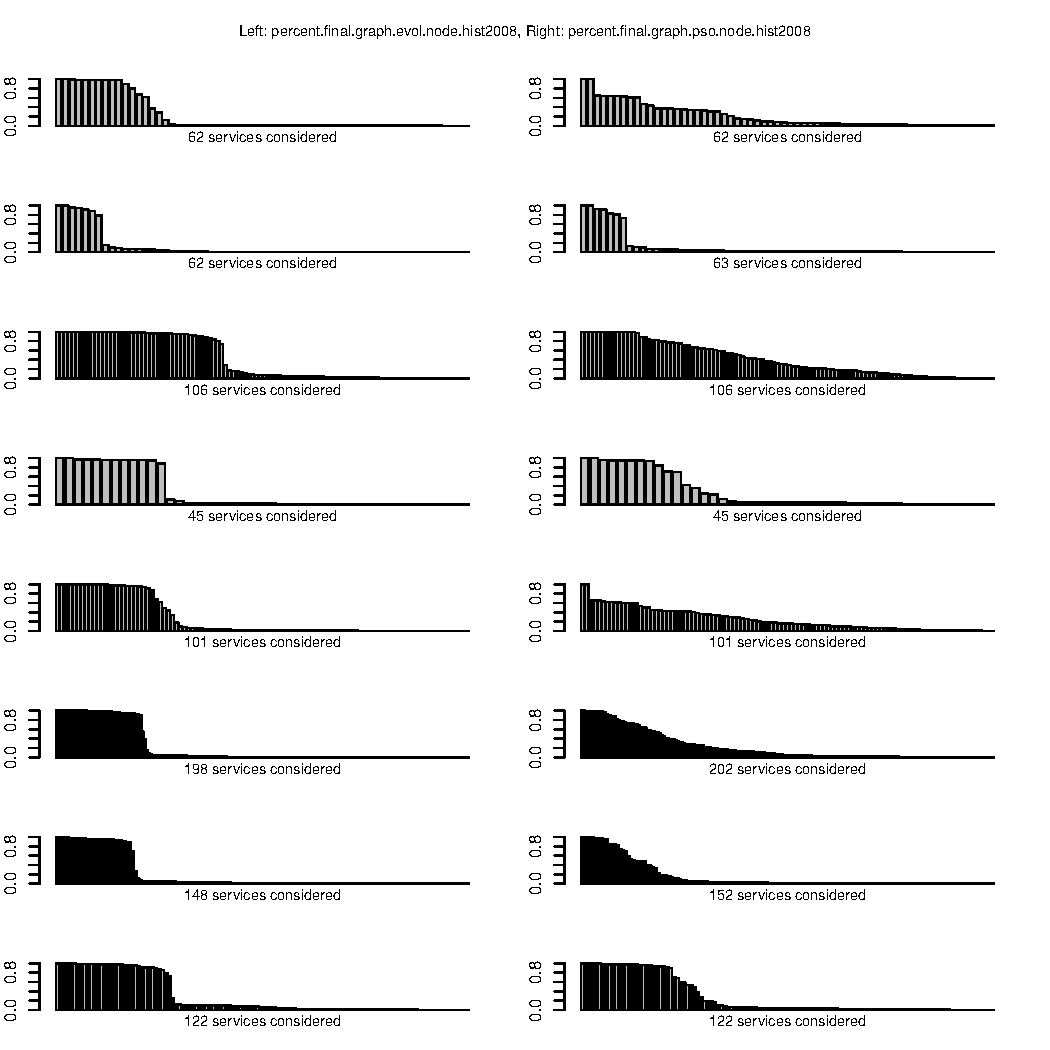
\includegraphics[width=10cm]{node_plots_run1_2008.pdf}}}
 \caption{Bar charts showing the frequency with which atomic services appear in solutions, for WSC 2008 datasets.}
 \label{bar_charts2008}
\end{figure}

\begin{figure}[h]
\centerline{
\fbox{
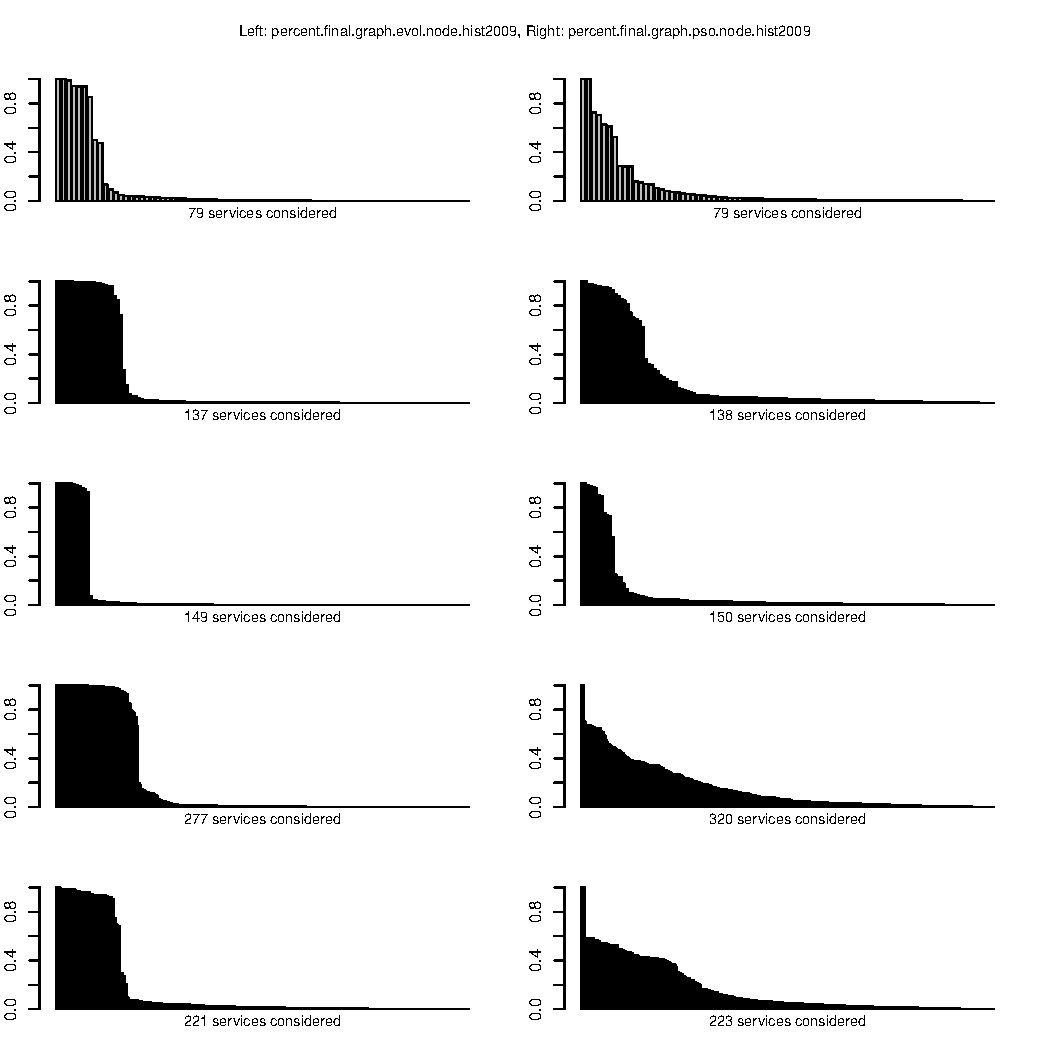
\includegraphics[width=10cm]{node_plots_run1_2009.pdf}}}
 \caption{Bar charts showing the frequency with which atomic services appear in solutions, for WSC 2009 datasets.}
 \label{bar_charts2009}
\end{figure}

\section{Analysis of Results}

The fitness results presented in Table \ref{tab:results} generally show that the solution fitness produced by the PSO-based approach is equivalent to that of the graph-based approach. However, it must also be noted that the fitness of solutions is significantly higher for the PSO-based approach in a number of datasets (3, 6, and 7 of WSC 2008, and 4 of WSC 2009), whereas this is only the case for the graph-based approach when using dataset 5 of WSC 2009. Thus, these results indicate that the PSO-based approach is preferrable when the focus of the composition process is on the quality of the resulting solutions. This conclusion is supported by the bar graphs produced when running each dataset, which show that PSO explores the inclusion of different atomic services in a more ``spread'' way than the graph-based approach for all datasets. Namely, the frequencies with which services appear in graph-based solutions are either very high or very low, indicating that this approach converges to a small area of the search space relatively quickly. In the PSO-based approach, on the other hand, the atomic service frequencies lower gradually, showing that a larger area of the search space was considered.

Finally, with regards to the execution time of the two techniques, it is clear that the PSO-based approach is more time-consuming than the graph-based approach. This is the case for two reasons: firstly, the PSO-based approach must decode solutions before every fitness evaluations, which involves the time-consuming steps of sorting the service queue and building an entirely new graph; secondly, the queue must be traversed repeatedly when building the corresponding graph. Even though the graph-based approach also requires some graph reconstruction, it relies on a shorter queue of services that is gradually populated with relevant candidates, thus resulting in a more efficient execution.

\section{Conclusion}\label{conclusion}

This work introduced a PSO-based QoS-aware Web service composition approach that relies on an indirect solution representation, as opposed to the direct representations used by current works in the area. The key idea of this approach is to optimise a queue of candidate atomic services, identifying the sequence that leads to the construction of a composition with the highest possible quality. In order to evaluate the quality of a candidate, the queue is fed into an algorithm that builds a directed acyclic graph (DAG) representing a service composition, which is then used in fitness calculations. This PSO-based approach was compared to a graph-based approach with direct solution representation, with results showing that the quality of the solutions produced by PSO generally matches or surpasses those produced by the graph-based approach, even though PSO requires a longer execution time. Additionally, tracking of the appearance of atomic services in solutions throughout the run showed that PSO explores the search space more effectively than its graph-based counterpart. Future work to this approach should investigate ways of reducing the execution time required when decoding solutions from the particles, by considering alternative particle representations and improved algorithms for building DAGs from service queues.

\bibliographystyle{splncs03}
\bibliography{bibliography}

\end{document}